% !TeX root = main.tex
% ============================================================
%  封面：李思风（极简学术）—— 白底、居中标题、无装饰边框
%  中部线稿改为「代码编辑器窗口」简笔，替换模板的数学函数曲线
%
%  可用字段（在 main.tex 导言区 \newcommand 预定义即可覆盖）：
%    \notename      主标题（必填）
%    \noteauthor    作者（必填）
%    \notesubtitle  标题下方小字，默认 \today
%    \noteextra     底部单位行，默认不显示
% ============================================================
\begin{titlepage}
	\thispagestyle{empty}
	\providecommand{\notesubtitle}{\today}
	\providecommand{\noteextra}{}
	\begin{center}
		\vspace*{4.7cm}

		% ---- 主标题 ----
		{\bfseries\songti\fontsize{24.8}{30}\selectfont \notename\par}

		\vspace{4.1cm}

		% ---- 日期 / 版本行 ----
		{\songti\fontsize{14.4}{18}\selectfont （\notesubtitle）\par}

		\vspace{3.4cm}

		% ---- 简笔线稿：编辑器窗口（可整段删除）----
		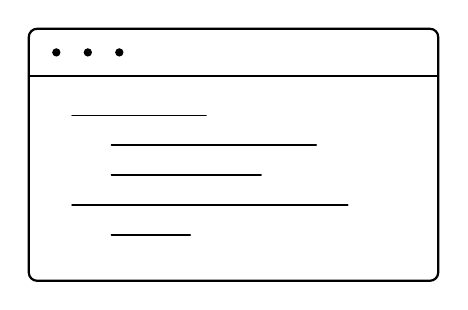
\begin{tikzpicture}[line width=0.8pt, line cap=round]
			% 窗口外框
			\draw[rounded corners=3pt] (-2.6,-1.6) rectangle (2.6,1.6);
			% 标题栏分隔线
			\draw[line width=0.6pt] (-2.6,1.0) -- (2.6,1.0);
			% 标题栏三个圆点
			\fill (-2.25,1.3) circle (1.5pt);
			\fill (-1.85,1.3) circle (1.5pt);
			\fill (-1.45,1.3) circle (1.5pt);
			% 代码行（长短不一，模拟缩进层次）
			\draw[line width=0.6pt] (-2.05,0.5) -- (-0.35,0.5);
			\draw[line width=0.6pt] (-1.55,0.12) -- (1.05,0.12);
			\draw[line width=0.6pt] (-1.55,-0.26) -- (0.35,-0.26);
			\draw[line width=0.6pt] (-2.05,-0.64) -- (1.45,-0.64);
			\draw[line width=0.6pt] (-1.55,-1.02) -- (-0.55,-1.02);
		\end{tikzpicture}

		\vspace{4.3cm}

		% ---- 作者（楷体）----
		{\kaishu\fontsize{24.8}{30}\selectfont \noteauthor\par}

		\vspace{1.8cm}

		% ---- 单位 / 学院（未定义则不显示）----
		{\songti\fontsize{20.7}{26}\selectfont \noteextra\par}

		\vspace*{1.6cm}
	\end{center}
\end{titlepage}
